\documentclass[a4paper,11pt]{article}

\usepackage[spanish]{babel}
\usepackage[utf8]{inputenc}
\usepackage{hyperref}
\usepackage{graphicx}
\usepackage{amsmath}
\usepackage{amsfonts}
\graphicspath{{images/}} 

\author{Daniel Monjas Miguélez}
\title{FR: Tema 2}

\begin{document}
\begin{titlepage}
\centering
    \vfill
    {\bfseries\Large
        Fundamentos de Redes: Tema 3\\
        10 de Octubre del 2020\\
        A year to Forget \\
        \vskip2cm
        Daniel Monjas Miguélez\\
    }    
    \vfill
    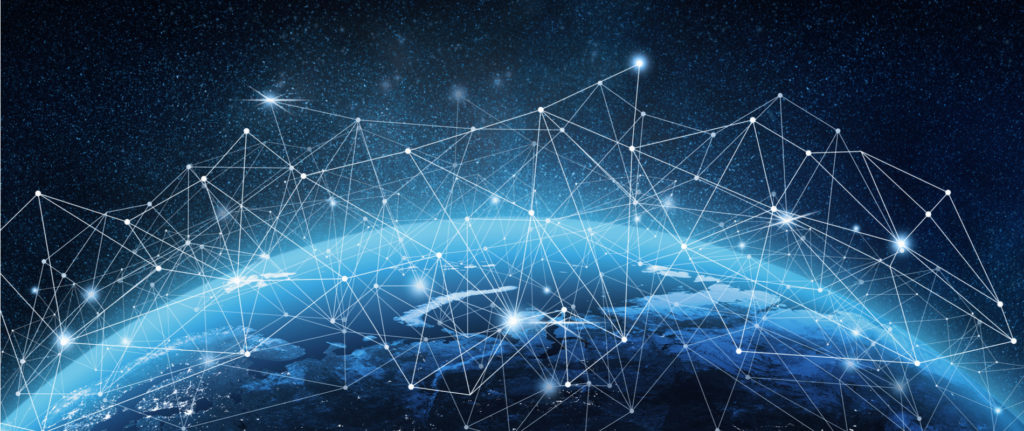
\includegraphics[width=15cm]{redes.jpg}
    \vfill
    \vfill
\end{titlepage}

\newpage
\tableofcontents
\newpage

\section{Introducción}
Las principales funciones y servicios suministrados por la capa de transporte son comunicación extremo a extremo (end-to-end) y la multipleación/demultiplexación de aplicaciones, lo que implica el uso de puertos. \\

Se denomina demultiplexación a la acción de entregar los datos contenidos en un segmento de la capa de transporte al socket correcto. Por el contrario, a la tarea de reunir los fragmentos de datos en el host de origen desde los diferentes sockets, encapsulando cada fragmento de datos con la información de cabecera (la cual luego se usa en la demultiplexación) para crear segmentos y pasarlos a la capa de red es lo que se denomina multiplexación. \\

Basándoonos en las explicaciones anteriores, sabemos que la operación de multiplexación que se lleva a cabo en la capa de transporte requiere que los sockets tenga identificadores únicos y que cada segmento tenga campos especiales que indiquen el socket al que tiene que entregarse el segmento. Estos campos especiales son el \textbf{número de puerto origen} y el \textbf{número de puerto destino}, donde cada número de puerto es un número de 16 bits comprendido en el rango de 0 a 65535. Los números comprendidos entre 0 y 1023 se conocen como \textbf{número de puertos bien conocidos} y son restringidos, lo que significa que están reservados para ser empleados por los protocolos de aplicación bien conocidos. \\

Tanto el protocolo TCP como el UDP proporcionan la multiplexación/demultiplexación de aplicaciones. Ahora bien mientras que el protocolo UDP es un no orientado a conexión y no fiable, el protocolo TCP es orientado a conexión, fiable, con control de errores y flujo, control de conexión y control de congestión. \\

Finalmente en este tema también se abordarán las extensiones TCP.

\section{Protocolo de datagrama de usuario (UDP).}
UDP hace casi lo mínimo que un protocolo de transporte debe hacer. Además de la función de multiplexación/demultiplexación y de algún mecanismo de comprobación de errores, no añade nada a IP. UDP toma los mensajes procedentes del proceso de la aplicación, asocia los campos correspondientes a los números de puerto de origen y de destino para proporcionar el servicio de multiplexación/demultiplexación, añade dos campos pequeños más y pasa el segmento resultante a la capa de red. La capa de red encapsula el segmento de la capa de transporte en un datagrama IP y luego hace el mejor esfuerzo por entregar el segmento al host receptor. Obsérvese que UDP es un protocolo sin conexión luego no hay fase de establecimiento de la conexión entre las entidades. \\

Algunas aplicaciones están mejor adaptadas a UDP por las siguientes razones:

\begin{itemize}
\item \textit{Mejor control en el nivel de aplicación sobre qué datos se envían y cuando}. Con UDP, tan pronto como un proceso de la capa de aplicación pasa datos a UDP, este los empaqueta en un segmento UDP e inmediatamente entrega el segmento a la capa red. Por el contrario, TCP dispone de un mecanismo de control de congestión que regula el flujo del emisor TCP en la capa de transporte cuando uno o más de los enlaces existente entre los hosts de origen y de destino están excesivamente congestionados.

\item \textit{Sin establecimiento de la conexión.} Ya hemos hablado de que TCP lleva un proceso de establecimiento de conexión, el cual consta de tres fases, antes de inicial la transferencia de datos. UDP inicia la transmisión sin formalidades preliminares. Por tanto, UDP no añade ningún retardo a causa del establecimiento de una conexión. 

\item \textit{Sin información del estado de la conexión.} TCP mantiene información acerca del estado de la conexión en los sistemas terminales. En el estado de la conexión incluye información acerca de los buffers de recepción y envía, de los parámetros de control de congestión y de los parámetros relativos al número de secuencia y de reconocimiento. Por el contrario, UDP no mantiene información del estado de la conexión y no controla ninguno de estos parámetros. Por esta razón, un servidor dedicado a un aplicación concreta suele poder soportar más clientes activos cuando la aplicación se ejecuta sobre UDP que cuando lo hace sobre TCP.

\item \textit{Poca sobrecarga debida a la cabecera de los paquetes.} Los segmentos TCP contienen 20 bytes en la cabecera de cada segmento, mientras que UDP solo requiere 8 bytes.
\end{itemize}

La ausencia de un mecanismo de control de congestión UDP puede dar lugar a altas tasas de pérdidas entre un emisor y un receptor UDP y al estrangulamiento de las sesiones TCP. Además cabe descargar que cuando se hacen envíos con UDP no hay garantías de recepción ordenada.

\begin{figure}[h]
\centering
\caption{Estructura de la cabecera de UDP y de la demultiplexación}
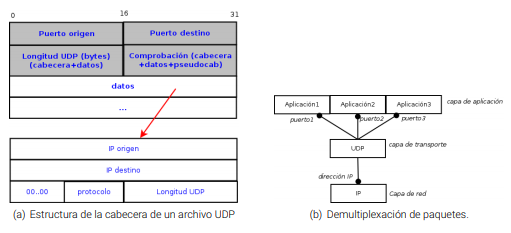
\includegraphics[scale=1,width=1.1\textwidth]{cabecera_udp.png}
\end{figure}

\subsection{Estructura de los segmentos UDP.}
Los datos de la aplicación ocupan el campo de datos del segmento UDP. La cabecera UDP solo tiene cuatro campo, y cada uno de ellos tiene un longitud de dos bytes. Como se ha explicado en la sección anterior, los números de puerto permiten al host de destino pasar los datos de la aplicación al proceso apropiado que está ejecutándose en el sistema terminal de destino. El campo de longitu especifica el número de bytes del segmento UDP (la cabecera más los datos). Es necesario un valor de longitud explícito ya que el tamaño del campo de datos puede variar de un segmento UDP al siguiente. El host recepto utiliza la suma de comprobación  ('\textit{checksum}') para detectar si se han introducido errores en el segmento. En realidad, la suma de comprobación también se calcula para unos pocos campos de la cabecera IP, además de para el segmento UDP. \\

\subsection{Suma de comprobación de UDP.}
La suma de comprobación UDP proporciona un mecanismo de detección de errores. Es decir, se utiliza para determinar si los bits contenidos en el segmento UDP han sido alterados según se desplazaban desde el origen al destino. UDP en el lado del emisor calcula el complemento a 1 de la suma de todas las palabras de 16 bits del segmento, acarreando cualquier desbordamiento obtenido durante la operación de suma sobre el bit de menor peso. Este resultado se almacena en el campo suma de comprobación del segmento UDP. En el receptor, las cuatro palabras de 16 bits se suman, incluyendo la suma de comprobación. Si no se han producido errores en el paquete, entonces la suma en el receptor tiene que ser todo unos. Si hay algún 0, entonces sabemos que el paquete contiene errores. \\

UDP proporciona la suma de comprobación, a pesar de que muchos protocolos de la capa de enlace proporcionan mecanismos de comprobación de errores, pues no existe ninguna garantía de que todos los enlaces existentes entre el origen y el destino proporcionen un mecanismo de comprobación de errores; es decir, uno de los enlaces puede utilizar un protocolo de la capa de enlace que no proporciones comprobación de errores. Además, incluso si los segmentos se transfieren correctamente a través del enlace, es posible que se introduzcan errores de bit cuando un segmento se almacena en la memoria de un router. Dado que no están garantizadas ni la fiabilidad de enlace, ni la detección de errores durante el almacenamiento en memoria, UDP tiene que proporcionar un mecanismo de detección de errores, terminal a terminal, si el servicio de transferencia de datos terminal a terminal ha de proporcionar la detección de errores.

Dado que IP está pensado para ejecutarse sobre prácticamente cualquier protocolo de la capa 2, resulta útil para la capa de transporte proporcionar un mecanismo de comprobación de errores como medida de seguridad. Aunque UDP proporciona este mecanismo, no hace nada para recuperarse del error. Algunas implementaciones de UDP simplemente descartan el segmento dañado y otras lo pasan a la aplicación con una advertencia. \\

\begin{figure}
\centering
\caption{Aplicaciones de internet populares y sus protocolos de transporte subyacentes}
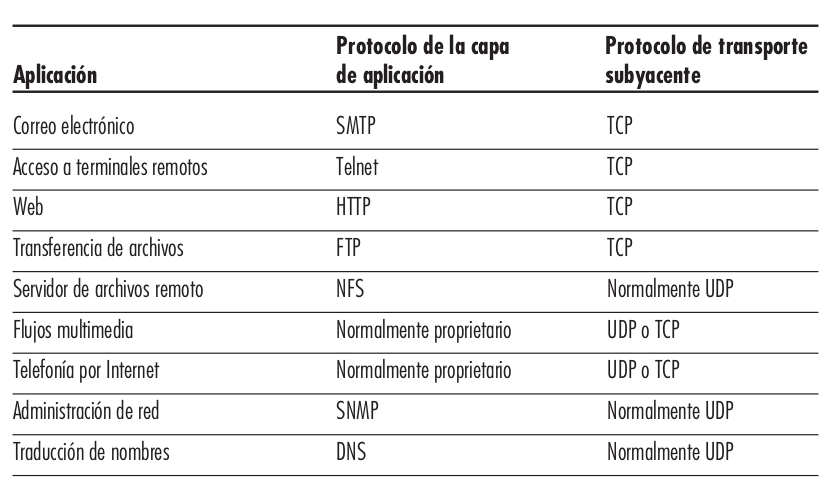
\includegraphics[scale=1,width=0.8\textwidth]{procolos_udp.png}
\end{figure}

Lo normal cuando un desarrollador de aplicaciones crea un socket UDP es que a este se le asigna un número de puerto libre en el rango 1024 a 65535 que esté libre (siempre que no se especifique uno). Por otro lado, si el desarrollador estuviera implementando el lado del servidor de un 'protocolo bien conocido', entonces tendría que asignar el correspondiente número de puerto bien conocido. Normalmente, el lado del cliente de la aplicación permite a la capa de transporte asignar de forma automática (y transparente) el número de puerto, mientras que el lado de servidor de la aplicación asigna un número de puerto específico.

\section{Protocolo de control de transmisión (TCP)}
TCP es un protocolo de la capa de transporte de internet, fiable y orientado a la conexión. Se dice que TCP está orientado a conexión porque antes de que un proceso de la capa de aplicación pueda comenzar a enviar datos a otro, los dos procesos deben primero 'establecer una comunicación' entre ellos; es decir, tienen que enviarse ciertos segmentos preliminares para definir los parámetros de la transferencia de datos que van a llevar a cabo a continuación. \\

La conexión TCP es una conexión lógica, con un estado común que reside solo en los niveles TCP de los sistemas terminales que se comunicacn. Dado que este protocolo se ejecuta únicamente en los sistemas terminales, los elemento intermedios de la red no mantienen el estado de la conexión TCP.

Una conexión TCP proporciona un servicio full-duplex y es casi siempre punto a punto, es decir, un único emisor y un único receptor. Cuando se establece una conexión TCP se hace por medio de un procedimiento denominado acuerdo en tres fases. También incluye un mecanismo de control de flujo de detección y recuperación de errores denominado ARQ (\textit{Automatic Repeat reQuest}) donde se usan dos cosas fundamentales: confirmaciones positivas que son paquetes de control que permiten controlar cuándo  ha llegado un segmento a la otra dirección, los paquetes que se usan para confirmar se denominan ACK. No se usan confirmaciones negativas para indicar que un paquete ha llegado mal o no ha llegado, sino que el emisor cada vez que manda un paquete inicia un temporizador, si al finalizar dicho temporizador no ha recibido confirmación vuelve a enviar el paquete. \\

Una vez que se ha establecido una conexión TCP, los dos procesos de aplicación pueden enviarse datos entre sí. El proceso cliente pasa un flujo de datos a través del socket (la puerta del proceso). Una vez que los datos atraviesan la puerta, se encuentran en manos del protocolo TCP que se ejecuta en el cliente. TCP dirige estos datos al buffer de emisión de la conexión, que es uno de los buffers que se definen durante el acuerdo de tres fases.

\begin{figure}[h]
\centering
\caption{Buffers de emisión y recepción de TCP}
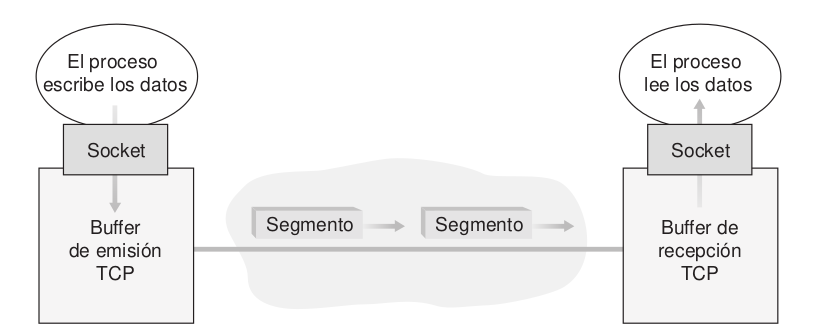
\includegraphics[scale=1,width=0.8\textwidth]{buffer_emision.png}
\end{figure}

De vez en cuando, TCP tomará fragmentos de datos del buffer de emisión y los pasa a la capa de red. La cantidad máxima de datos que pueden escogerse y colocarse en un segmento está limitada por el tamaño máximo de segmento (\textbf{MSS, \textit{Maximum Segment Size}}). Normalmente, el MSS queda determinado por la longitud de la trama más larga de la capa de enlace que el host emisor local puede enviar (\textbf{Maximum Transmission Unit (MTU)}), y luego el MSS se establece de manera que se garantice que un segmento TCP más la longitud de la cabecera TCP/IP (normalmente 40 bytes) se ajuste a una única trama de la capa de enlace. \\

TCP empareja cada fragmento de datos del cliente con una cabecera TCP, formando segmentos TCP. Los cuales se pasan a la capa de red, que los encapsula por separado dentro de datagramas IP de la capa de red. Cada lado de la conexión tiene su propio buffer de emisión y su propio buffer de recepción. \\

Por tanto, una conexión TCP consta de buffers, variables y un socket de conexión a un proceso en un host, y otro conjunto de buffers, variables y un socket de conexión a un proceso en otro host. \\

\subsection{Estructura del segmento TCP}
El segmento TCP consta de campos de cabecera y un campo de datos. El campo de datos contiene un fragmento de los datos de aplicación. Como ya hemos mencionado, el MSS limita el tamaño máximo del campo de datos de un segmento. Cuando TCP envía un archivo grande, normalmente divide el archivo en fragmentos de tamaño MSS. Sin embargo, las aplicaciones interactivas suelen transmitir fragmentos de datos que son más pequeños que el MSS. Habitualmente la cabecera de TCP tiene 20 bytes (12 bytes más que la cabecera de UDP).

\begin{figure}[h]
\centering
\caption{Estructura del segmento TCP}
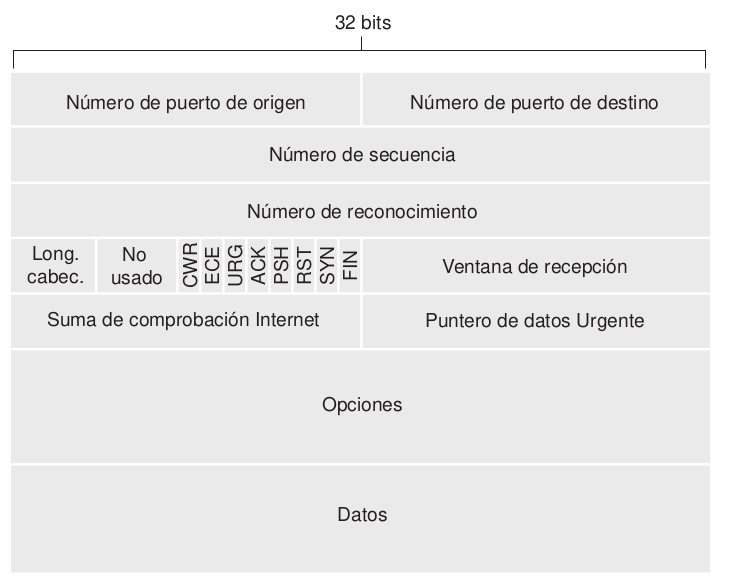
\includegraphics[scale=1,width=0.8\textwidth]{estructura_tcp.png}
\end{figure} 

Al igual que con UDP, la cabecera incluye los números de puerto origen y puerto de destino, que se utilizan para multiplexar y demultiplexar los datos de y para las aplicaciones de la capa superior. También, al igual que UDP, incluye un campo de suma de comprobación. A partes de estos, incluye también los siguientes campos:

\begin{itemize}
\item El campo número de secuencia de 32 bits y el campo número de reconocimiento también de 32 bits, que son utilizados por el emisor y el receptor de TCP para implementar un servicio de transferencia de datos fiable.

\item El campo ventana de recepción de 16 bits se utiliza para el control de flujo

\item El campo longitud de cabecera de 4 bits especifica la longitud de la cabecera TCP en palabras de 32 bits. La cabecera puede tener una longitud variable a causa del campo opciones de TCP (normalmente vacío, luego la longitud habitual de la cabecera TCP es 20 bytes).

\item El campo opciones es opcional y de longitud variable. Se utiliza cuando un emisor y un receptor negocian el tamaño máximo de segmento (MSS) o como un factor de escala de la ventana en las rede de alta velocidad. También se define una opción de marca temporal.

\item El campo Indicador tiene 6 bits. El bit ACK se utiliza para indicar que el valor transportado en el campo de reconocimiento es válido; es decir, el segmento contiene un reconocimiento apra un segmento que ha sido recibido correctamente. Los bits RST, SYN y FIN se utilizan para el establecimiento y cierre de conexiones. Los bits CWR y ECE se emplean en la notificación de congestión explícita. La activación del bit PSH indica que el recpetor deberá pasar los datos a la capa superior de forma inmediata. Por último, el bit URG se utiliza para indicar que hay datos en este segmento que la entidad de la capa superior del lado del emisor ha marcado como urgentes. La posición de este último byte de estos datos urgente se indica mediante el campo puntero de datos urgentes de 16 bits.
\end{itemize}

\textbf{Números de secuencia y números de reconocimiento.} Dos de los campos más importantes de la cabecera de un segmento TCP son el campo número de secuencia y el campo número de reconocimiento. Estos campos son una parte crítica del servicio de transferencia de datos fiable de TCP. \\

TCP percibe los datos como un flujo de bytes no estructurado pero ordenado. El uso de TCP de los números de secuencia refleja este punto de vista, en el sentido de que los números de secuencia hacen referencia al flujo de bytes transmitido y no a la serie de segmentos transmitidos. El número de secuencia de un segmento es por tanto el número del primer byte del segmento dentro del flujo de bytes. El número de secuencia inicial se escoge normalmente como un valor entero que incrementa su valor cada 4$\mu s$ aproximadamente, lo que nos daría un ciclo de 4 horas y 46 minutos.\\

Para explicar los números de reconocimiento se debe recordar que TCP es una conexión full-dupex, de modo que el host A puede estar recibiendo datos del host B mientras envía datos al host B. El número de reconocimiento que el host A incluye en su segmento es el número de secuencia del siguiente byte que el host A está esperando del host B. Un ejemplo: suponga que el host A ha recibido un segmento del host B que contiene los bytes de 0 a 535 y otro segmento que contiene los bytes de 900 a 1000. Por alguna razón, el host A no ha recibido los bytes de 536 a 899. En este ejemplo, el host A está esperando el byte 536 (y los que le siguen) para volver a crear el flujo de datos de B. Por tanto, el siguiente segmentod e A a B contendrá el número 536 en el campo de número de reconocimiento. Dado que TCP sólo confirma los bytes hasta el primer byte que falta en el flujo, se dice que TCP proporciona reconocimientos acumulativos.

\subsection{Gestión de la conexión TCP}
El proceso de aplicación cliente informa en primer lugar al cliente TCP que desea establecer una conexión con un proceso del servidor. A continuación, el protocolo TCP en el cliente establece una conexión TCP con el protocolo TCP en el servidor de la siguiente manera:

\begin{itemize}
\item \textit{Paso 1.} En primer lugar, TCP del lado del cliente envía un TCP especial al TCP del lado del servidor. Este segmento no contiene datos de la capa de aplicación. Pero uno de los bits indicadores de la cabecera del segmento, el bit SYN, se pone a 1. Además, el cliente selecciona de forma aleatoria un número de secuencia inicial y lo coloca en el campo número de secuencia del segemento TCP inicial SYN. Este segmento se encapsula dentro de un datagrama IP y se envía al servidor. Es importante la elección del valor número de secuencia inical para evitar ciertos ataques de seguridad.

\item \textit{Paso 2.} Una vez que el datagrama IP que contiene el segmento SYN TCP llega al host servidor, el servidor extrae el segmento SYN del datagrama, asigna los buffers y variables TCP a la conexión y envía un segmento de conexión concedida al cliente TCP. Este segmento tampoco contiene datos de la capa de aplicación. Sin embargo, contiene tres fragmentos de información importantes de la cabecera del segmento. El primero, el bit SYN se pone a 1. El segundo, el campo reconocimiento de la cabecera del segmento TCP se iguala al número de secuencia inicial recibido más uno. Por último, se elige su propio número de secuencia inicial y este valor se almacena en el campo número de secuencia del segmento TCP. Este segmento de conexión concedida se conoce como segmento SYNACK.

\item \textit{Paso 3.} Al recibir el segmento SYNACK, el cliente también asigna buffers y variables de conexión. El host cliente envía entonces al servidor otro segmento; este último confirma el segmento de conexión concedida del servidor. El bit SYN se pone a cero, ya que la conexión está establecida. Esta tercera etapa puede transportar datos del cliente al servidor dentro de la carga útil del segmento.
\end{itemize}

\begin{figure}[h]
\centering
\caption{El proceso de acuerdo en tres fases de TCP: intercambio de segmentos}
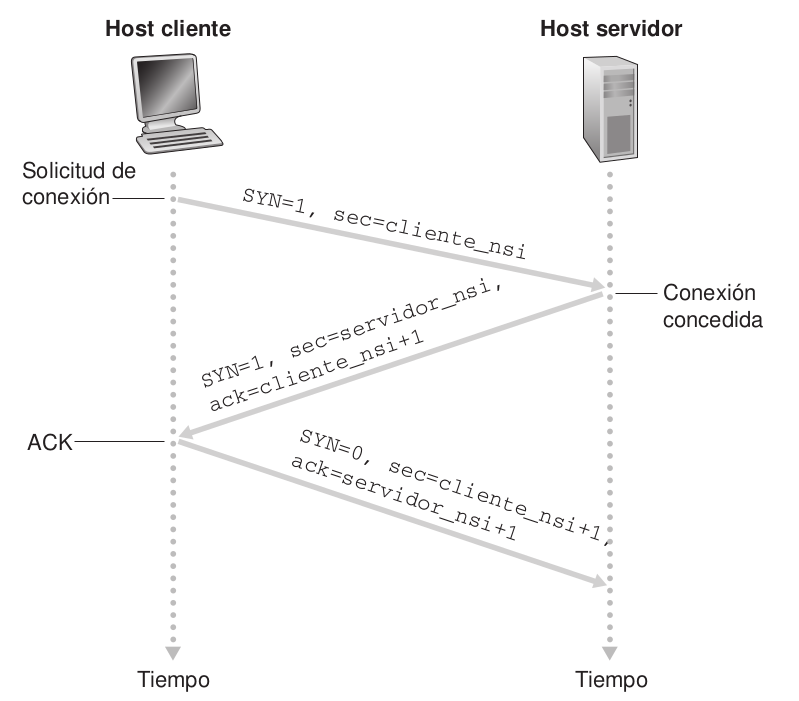
\includegraphics[scale=1,width=0.8\textwidth]{conexion_tcp.png}
\end{figure}

Cualquiera de los dos procesos participantes en una conexión TCP pueden dar por terminada dicha conexión. Cuando una conexión se termina, los 'recursos' de los host se liberan. El proceso de aplicación cliente ejecuta un comando de cierre. Esto hace que el cliente TCP envíe un segmento especial TCP al proceso servidor. Este segmento especial contiene un bit indicador en la cabecera del segmento, el bit FIN, puesto a 1. Cuando el servidor recibe este segmento, devuelve al cliente un segmento de reconocimiento. El servidor entonces envía su propio segmento de desconexión, que tiene el bit FIN puesto a 1. Por último, el cliente reconoce el segmento de desconexión del servidor. En esta situación, los recursos de ambos hosts quedan liberados. \\

\begin{figure}[h]
\centering
\caption{Cierre de una conexión TCP}
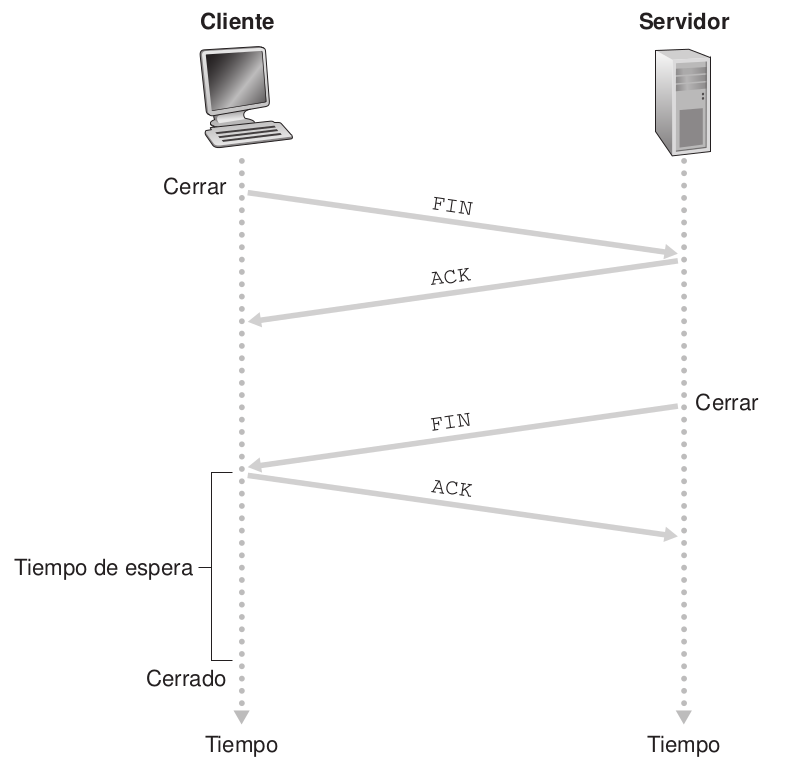
\includegraphics[scale=1,width=0.8\textwidth]{ejemplo_desconexion.png}
\end{figure}

Mientras se mantiene una conexión TCP, el protocolo TCP que se ejecuta en cada host realiza transiciones a través de los diversos estados TCP. La aplicación cliente inicia una nueva conexión, esto hace que TCP en el cliente envíe un segmento SYN a TCP en el servidor. Después de haber enviado el segmento SYN, el cliente TCP entra en el estado SYN\_SENT. Mientras se encuentra en este estado, el cliente TCP espera un segmento procedente del TCP servidor que incluya un reconocimiento del segmento anterior del cliente y que tenga el bit SYN puesto a 1. Una vez recibido ese segmento, el cliente TCP entra en el estado ESTABLISHED. Mientras está en este, el cliente TCP puede enviar y recibir segmentos TCP que contengan datos de carga útil. \\

Suponga que la aplicación cliente decide cerrar la conexión. Así, el cliente TCP envía un segmento TCP con el bit FIN  a 1 y entra en el estado FIN\_WAIT\_1. En este estado, el cliente TCP queda a la espera de un segmento TCP del servidor que contenga un mensaje de reconocimiento. Cuando lo recibe, el cliente entra en el estado FIN\_WAIT\_2. En este, el cliente espera a recibir otro segmento del servidor con el bit FIN puesto a 1; una vez recibido, el cliente TCP reconoce el segmento del servidor y pasa al estado TIME\_WAIT, en el que puede reenviar al cliente TCP el reconocimeinto final en caso de que el paquete ACK se pierda. El tiempo invertido en el estado TIME\_WAIT es dependiente de la implementación, siendo sus valores atípicos 30 segundos, 1 minuto y 2 minutos.

\begin{figure}[h]
\centering
\caption{Diagrama Estados TCP}
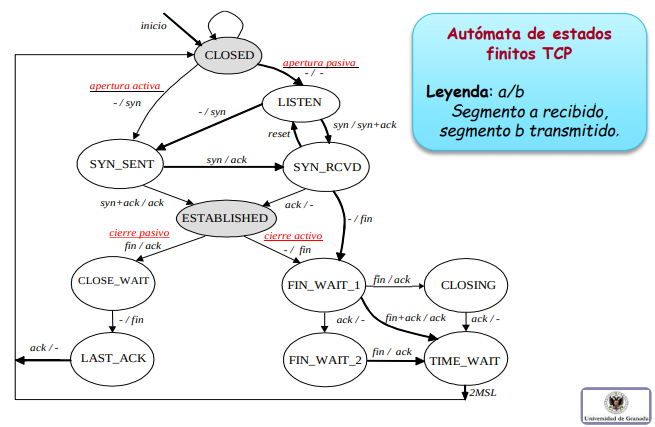
\includegraphics[scale=1,width=1\textwidth]{diagrama_tcp.png}
\end{figure}

En todos estos casos se ha supuesto que la conexión TCP se establece en un puerto correcto. Para explorar un puerto TCP específico, por ejemplo, el puerto 6789, en un host objetivo, nmap enviará un segmento TCP SYN con el puerto de destino 6789a dicho host. Puede obtenerse entonces tres posibles resultados:

\begin{itemize}
\item \textit{El host de origen recibe un segmento TCP SYNACK del host objetivo.} Dado que esto significa que hay una aplicación ejecutándose con TCP en el puerto 6789 del host objetivo, nmap devuelve 'open' (puerto abierto).

\item \textit{El host de origen recibe un segmento TCP RST procedente del host objetivo.} Esto significa que el segmento SYN ha alcanzado el host objetivo, pero este no está ejecutando una aplicación con TCP en el puerto 6789. Pero el atacante sabrá como mínimo que el segmento destinado al puerto 6789 del host no está bloqueado por ningún cortafuegos existente en la ruta entre los hosts de origen y de destino.

\item \textit{El origen no recibe nada.} Probablemente, esto significa que el segmento SYN fue bloqueado por un cortafuegos intermedio y nunca llegó al host objetivo.
\end{itemize}

\subsection{Estimación del tiempo de ida y vuelta y fin de temporización.}
TCP utiliza un mecanismo de fin de temporización/retransmisión para recuperarse de la pérdida de segmentos. Evidentemente, el intervalo de fin de temporización debería ser mayor que el tiemo de ida y vuelta (RTT) de la conexión; es decir, mayor que el tiempo que transcurre desde que se envía un segmento hasta que se recibe su reconocimiento. \\

\textbf{Estimación del tiempo de ida y vuelta.} El RTT de muestra, espresado como $RTTMuestra$, para un segmento es la cantidad de tiempo que transcurre desde que se envía el segmento hasta que se recibe el correspondiente paquete de reconocimiento del segmento. La mayor parte de implementaciones TCP toman solo una medida de $RTTMuestra$ cada vez. Es decir, en cualquier instante, $RTTMuestra$ se estima a partir de uno solo de los segmentos transmitidos pero todavía no reconocidos, lo que nos proporciona un nuevo valor de $RTTMuestra$ aproximadamente cada RTT segundos. \\

Obviamente, los valores de $RTTMuestra$ fluctuarán de un segmento a otro a causa de la congestión en los routers y a la variación de la carga en los sistemas terminales. Con el fin de estimar un RTT típico, TCP mantiene un valor promedio, $RTTEstimado$, de los valores de $RTTMuestra$. Para obtener dicho valor TCP utiliza la siguiente fórmula:

\begin{equation*}
RTTEstimado = (1-\alpha)\cdot RTTEstimado + \alpha \cdot RTTMuestra
\end{equation*}

El valor recomendado para $\alpha$ es $\alpha=0.125$. Obsérvese que $RTTEstimado$ es una media ponderada de los valores de $RTTMuestra$.

\begin{figure}[h]
\centering
\caption{Muestreo de RTT y estimación de RTT}
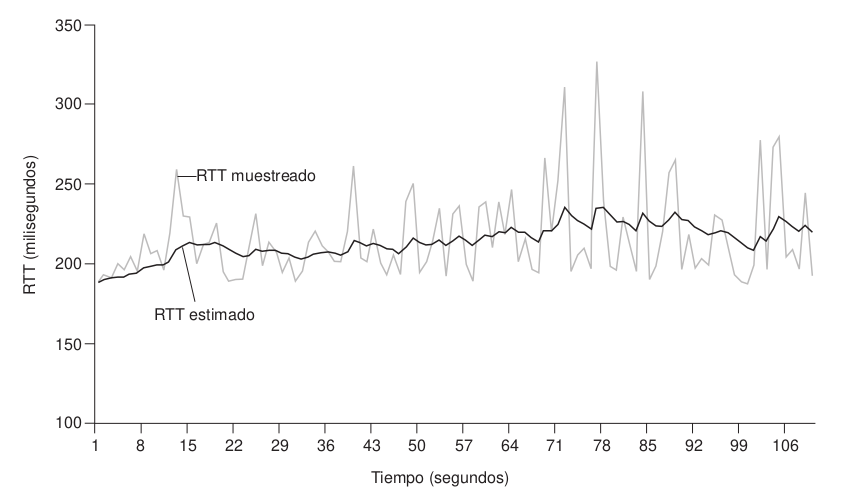
\includegraphics[scale=1,width=1.1\textwidth]{muestreo_rtt.png}
\end{figure}

Además de tener un estimado de RTT, también es importante disponder de una medida de la variabilidad de RTT. A esta la denominaremos $RTTDesv$, como una estimacińo de cuánto se desvía típicamente $RTTMuestra$ de $RTTEstimado$:

\begin{equation*}
RTTDesv =(1-\beta)\cdot RTTDesv + \beta \cdot |RTTMuestra - RTTEstimado|
\end{equation*}

Si los valores de $RTTMuestra$ presentan una pequeña fluctuación, entonces $RTTDesv$ será pequeño; por el contrario, si existe una gran fluctuación, $RTTDesv$ será grande. El valor recomendado para $\beta$ es 0.25. \\

\textbf{Definición y gestión del intervalo de fin de temporización para la retransmisión.} Lo deseable es que el intervalo de fin de temporización sea igual a $RTTMuestra$ más un cierto margen. Este margen deberá ser más grande cuando la fluctuación en los valores de $RTTMuestra$ sea más grande y más pequeño cuando la fluctuación sea pequeña. Todas estas consideraciones se tienen en cuenta en el método TCP para determinar el intervalo de fin de temporización de retransmisiones: 

\begin{equation*}
IntervaloFinTemporizacion = RTTEstimado + 4\cdot RTTDesv
\end{equation*}

Se recomienda que el valor inicial para $IntervaloFinTemporizacion$ sea de 1 segundo. \\

\textbf{Algunos escenarios interesantes.} El host A envía un segmento al host B. Ese segmento tiene el número de secuencia 92 y 8 bytes de datos. Después de enviar este segmento, el host A espera un segmento procedente de B con un número de reconocimiento de 100. Aunque el segmento se escirbe el  paquete de reconocimiento se pierde . Se produce un finde temporización y el host A retransmite el mismo segmento. El host B comprueba que los datos ya habían sido retransmitidos, los descarte y manda el ACK correspondiente.

\begin{figure}[h]
\centering
\caption{Retransmisión debida a la pérdida de un paquete de reconocimiento ACK.}
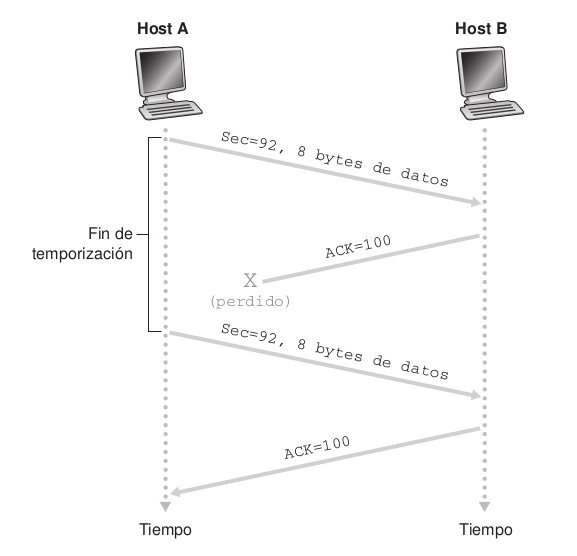
\includegraphics[scale=1,width=0.8\textwidth]{ejemplo_1.png}
\end{figure}

\textbf{Duplicación del intervalo de fin de temporización.} Examinemos alguna de las modificaciones que aplican la mayor parte de las implementaciones TCP. En esta modificación, cuando tiene lugar un suceso fin de temporarización TCP retransmite el segmento aún no reconocido con el número de secuencia más pequeño. Pero cada vez que TCP retransmite, define el siguiente intervalo de fin de temporización como dos veces el anterior, en lugar de obtenerlo a partir de los últimos valores de $RTTEstimado$ y $RTTDesv$. \\

\begin{figure}[h]
\centering
\caption{Segmento 100 no retransmitido}
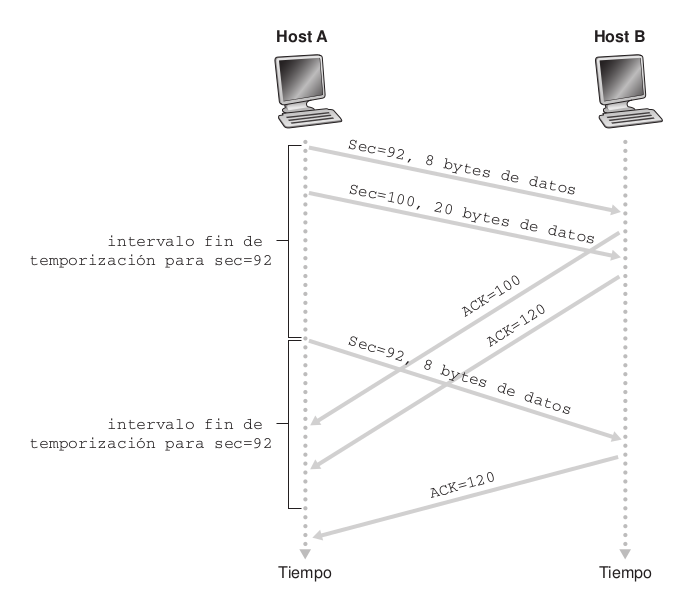
\includegraphics[scale=1,width=1\textwidth]{ejemplo_2.png}
\end{figure}

Esta modificación proporciona una forma limitada de control de congestión. La caducidad del temporizador está causada muy probablemente por la congestión de la red, es decir, llegan demasiados paquetes a una (o más) colas de router a lo largo de la ruta entre el origen y el destino, haciendo que los paquetes sean descartados y/o sufran largo retardos de cola. Cuando existe congestión, si los orígenes continúan retransmitiendo paquetes persistentemente, la congestión puede empeorar. En lugar de ello, TCP actúa de forma más diplomática, haciendo que los emisores retransmitan después de intervalos cada vez más grandes. \\

\begin{figure}[h]
\centering
\caption{Un reconocimiento acumulativo evita la retransmisión del primer segmento}
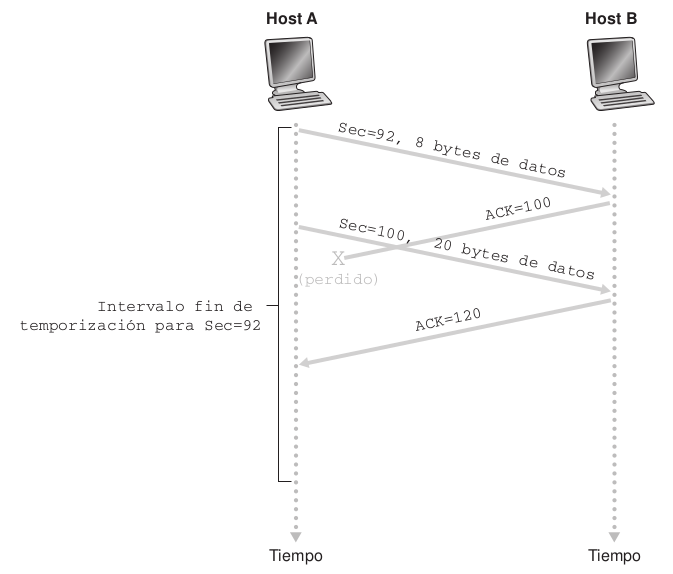
\includegraphics[scale=1,width=0.8\textwidth]{ejemplo_3.png}
\end{figure}

\textbf{Retransmisión rápida.} Uno de los problemas con las retransmisiones generadas por los sucesos de fin de temporización es que el periodo de fin de temporización puede ser relativamente largo. Un \textbf{ACK duplicado} es un ACK que vuelve a reconocer un segmento para el que el emisor ya ha recibido un reconocimiento anterior. Cuadno un receptor TCP recibe un segmento con un número de secuencia mayor que el siguiente número de secuencia en orden esperado, detecta un hueco en el flujo de datos, es decir, detecta que falta un segmento. Entonces el servidor simplemente vuelve a reconocer (es decir, genera un ACK duplicado) al último byte de datos en orden que ha recibido. \\

Puesto que un emisor suele enviar un gran número de segmentos seguidos, si se pierde uno de ellos, probablemente habrá muchos ACK duplicados seguidos. Si el emisor TCP recibe tres ACK duplicados para los mismo datos, toma esto como una indicación de que el segmento que sigue al segmento que ha sido reconocido tres veces se ha perdido. En este caso, el emisor TCP realiza un retransmisión rápida, reenviando el segmento que falta antes de que caduque el temporizador de dicho segmento.

\begin{figure}
\centering
\caption{Retransmisión rápida: retransmisión del segmento que falta antes de que caduque el temporizador del segmento}
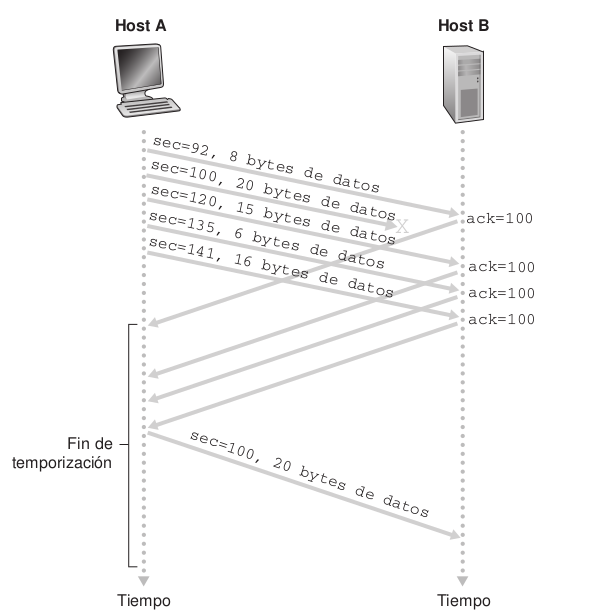
\includegraphics[scale=1,width=0.8\textwidth]{ejemplo_4.png}
\end{figure}

\begin{figure}
\centering
\caption{Recomendación para la generación de mensajes ACK en TCP}
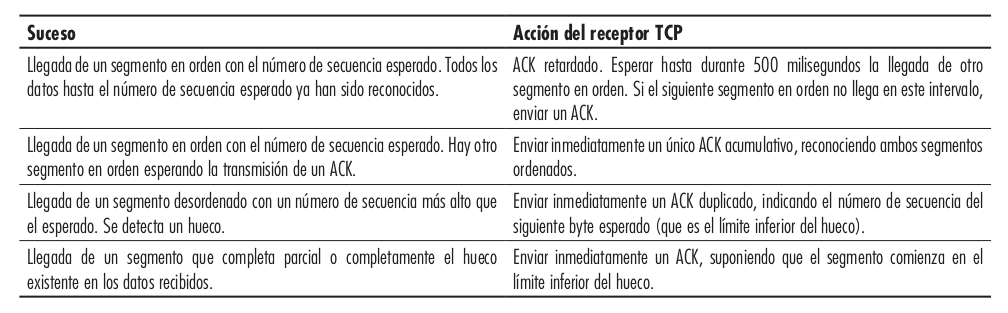
\includegraphics[scale=1,width=1.2\textwidth]{tabla_ack.png}
\end{figure}

\subsection{Control de flujo.}
TCP proporciona un servicio de control de flujo a sus aplicaciones para eliminar la posibilidad de que el emisor desborde el buffer del receptor. El control de flujo es por tanto un servicio de adaptación de velocidades. \\

TCP proporciona un servicio de control de flujo teniendo que mantienen el emisor una variable conocida como ventana de recepción. Informalmente, la ventana de recepción se emplea para proporcionar al emisor una idea de cuánto espacio libre hay disponible en el buffer del receptor.

\begin{equation*}
VentRecepcion=BufferRecepcion -[UltimoByteRecibido-UltimoByteLeido]
\end{equation*}

\begin{figure}[h]
\centering
\caption{La ventana de recepción (VentRecepcion) y el buffer de recepción (BufferRecepcion)}
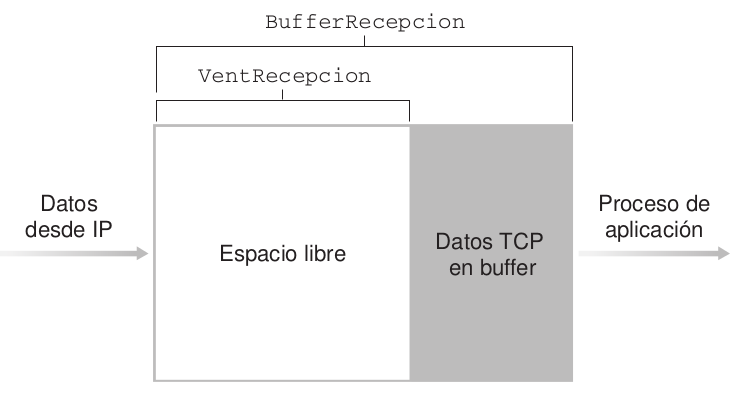
\includegraphics[scale=1,width=0.8\textwidth]{ventana_recepcion.png}
\end{figure}

\section{Control de congestión}
\subsection{Escenario 1: dos emisores, un router con buffers de capacidad ilimitada}
Sean dos hosts, A y B, cada uno de los cuales disponde de una conexión que comparte un único salto entre el origen y el destino.

Supongamos que la aplicación del host A está enviando datos a la conexión a una velocidad media de $\lambda_{in}$ bytes/segundo. Ignorando la sobrecarga adicional debida a la adición de la información de cabecera de las capas de transporte e inferiores, la velocidad a la que el host A entrega tráfico al reoute en este primer escenario es por tanto $\lambda_{in}$ bytes/segundo. El host B opera de forma similar, y suponemos que también está enviando a una velocidad de $\lambda_{in}$ bytes/segundo. Los paquetes que salen de los hosts A y B atraviesan un router y un enlace de salida compartido de capacidad R. \\

\begin{figure}[h]
\centering
\caption{Escenario de congestión 1: tasa de transferencia y retardo en función de la velocidad de transmisión del host}
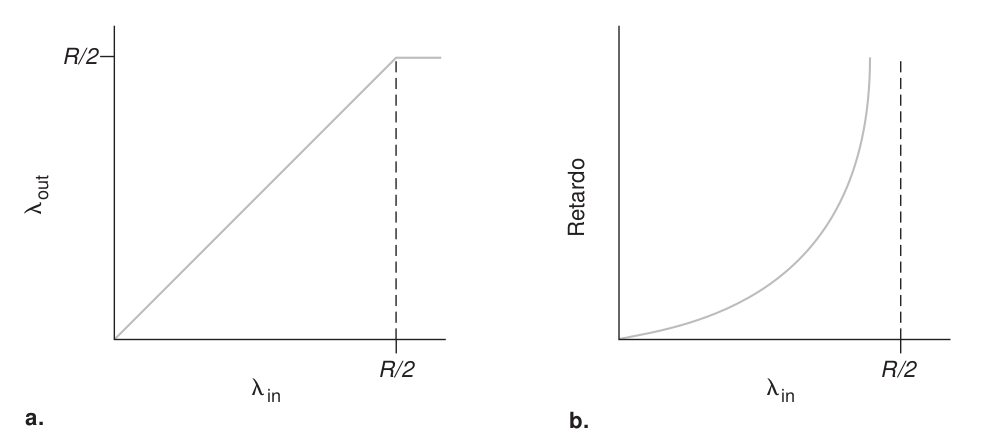
\includegraphics[scale=1,width=1\textwidth]{escenario_1.png}
\end{figure}

La gráfica a. de la figura 15 muestra la tasa de transferencia por conexión (número de bytes por segundo en el receptor) como una función de la velocidad de transmisión de la conexión. Para una velocidad de transmisión comprendida entre 0 y R/2, la tasa de transferencia en el receptor es igual a la velocidad de transmisión en el emisor. La gráfica de la derecha muestra la consecuencia de operar cerca de la capacidad de enlace. A medida que la velocidad se aproxima a R/2, el retardo medio se hace cada vez más grande. Cuando la velocidad de transmisión excede R/2, el número medio de paquetes en cola en el router no está limitado y el retardo medio entre el origen y el destino se hace infinito.

\subsection{Escenario 2: dos emisores y un router con buffers finitos.}
Ahora se supone que el espacio en los buffers es finito. Una consecuencia de esto es que los paquetes serán descartados cuando lleguen a un buffer ya lleno. Consideramos que las conexiones son fiables, es decir, si un paquete se descarta el transmisor lo retransmite. Vamos a designar la velocidad a la que la aplicación envía los datos originales al socker como $\lambda_{in}$ bytes/segundo. La velocidad a la que la capa de transporte envía segmentos $\lambda_{in}'$ bytes/segundo.

\begin{figure}[h]
\centering
\caption{Escenario 2: rendimiento con buffers de capacidad finita}
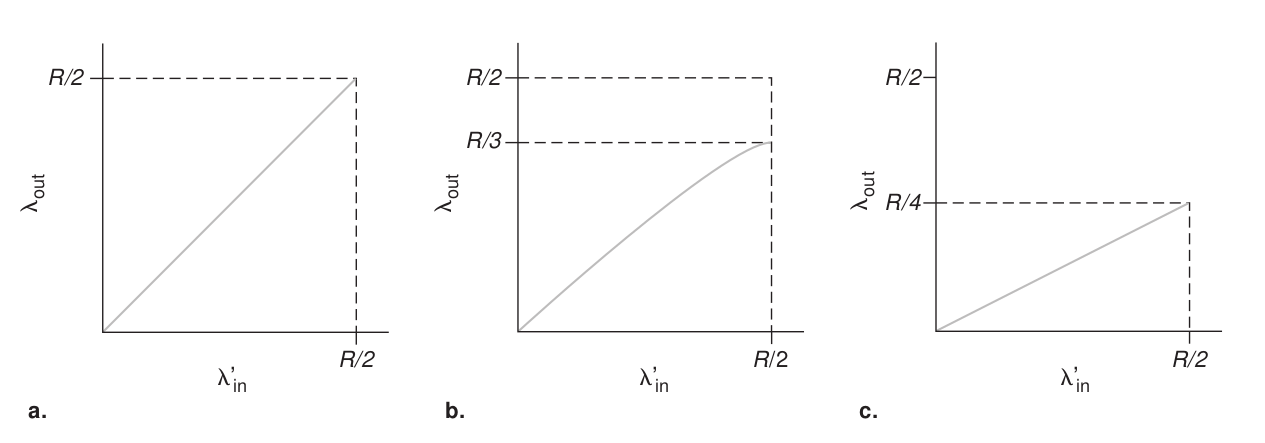
\includegraphics[scale=1,width=1\textwidth]{escenario_2.png}
\end{figure}

El rendimiento de este segundo escenario dependerá en gran medida de cómo se realicen las retransmisiones. La gráfica a. muestra el caso no realista en el que el host A es capaz de determinar si el buffer en el router está libre o lleno y enviar entonces un paquete sólo cuando el buffer esté libre. Consideremos ahora un caso más realista, donde el emisor solo retransmite con seguridad cuando sabe que un paquete se ha perdido. En este caso el rendimiento es similar al de la gráfica b. Para apreciar este caso considere que $\lambda_{in}'$ es R/2. Para este valor de la carga ofrecida la velocidad a la que los datos son suministrados a la aplicación del receptor es R/3. Por tanto, de las 0.5R unidades de datos transmitidos, 0.3333R bytes/segundo son datos originales y 0.166R bytes/segundo son retransmitidos. \\

Por último se considera el caso en el que el emisor puede alcanzar el fin de la temporización de forma prematura y retransmitir un paquete que ha sido retardado en la cola pero que todavía no se ha perdido. En este caso, el trabajo realizado por el router al reenviar la copia retransmitida del paquete original se desperdicia, ya que el receptor ya había recibido la copia original de ese paquete. Esto se muestra en la gráfica C, lo que nos dice que para una velocidad de transporte de R/2 la transferencia de datos a la aplicación receptora es sólo de R/4, ya que los R/3 restantes son utilizados en retransmitar paquetes retardados cuyo tiempo ha vencido, luego la media por paquete es retransmitirlo dos veces.

\subsection{Escenario 3: cuatro emisores, routers con buffers de capacidad finita y rutas con múltiples saltos.}
En este último escenario consideramos 4 hosts que transmiten paquetes a través de rutas solapadas con dos saltos. De nuevo suponemos que cada host utiliza un mecanismo de fin de temporización/retransmisión para implementar un servicio de transferencia de datos fiable, que todos los hosts tienen el mismo valor $\lambda_{in}$ y que todos los enlaces de router tienen una capacidad de R bytes/segundo.

\begin{figure}[h]
\centering
\caption{Cuatro emisores, routers con buffers finitos y rutas con varios saltos.}
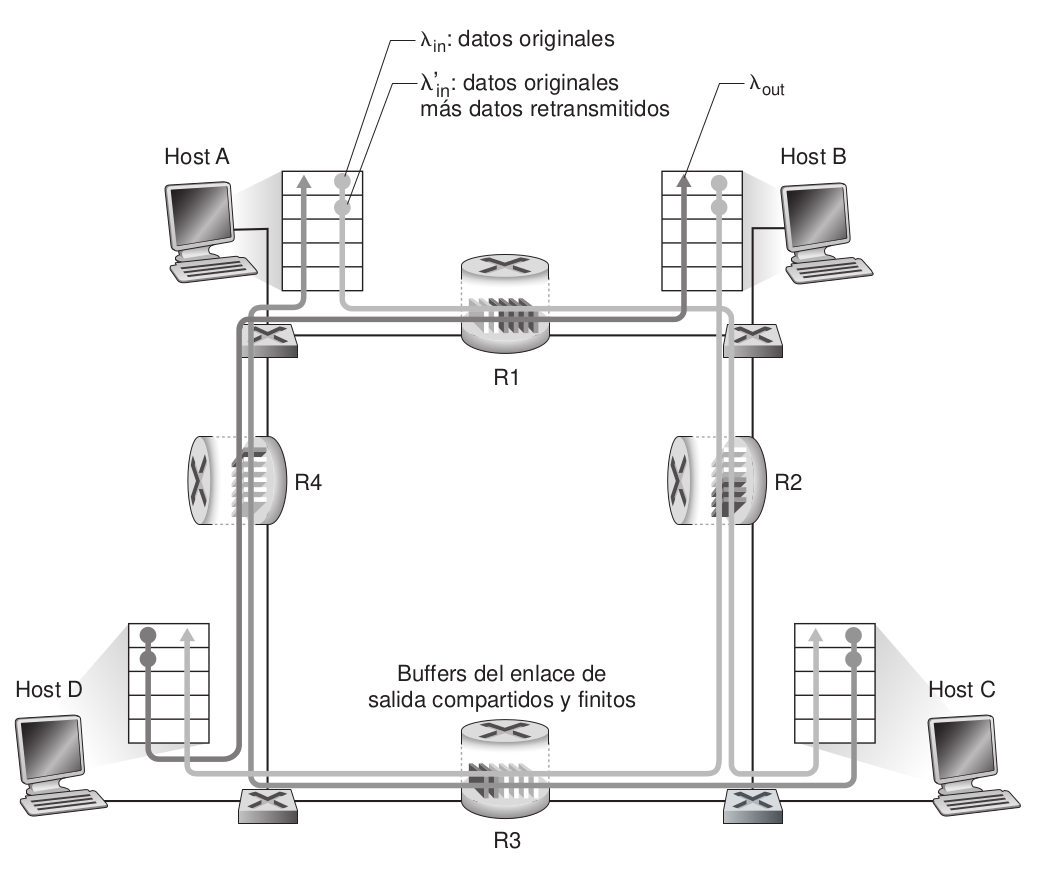
\includegraphics[scale=1,width=0.8\textwidth]{escenario_3.png}
\end{figure}

Para valores extremadamente pequeños de $\lambda_{in}$, es raro que el buffer se desborde, y la tasa de transferencia es aproximadamente igual a la carga ofrecida. Para valores ligeramente más grandes de $\lambda_{in}$, la correspondiente tasa de transferencia es también más grande, ya que se están transmitiendo más datos originales por la red y entregándose a su detino, y los desbordamientos siguen siendo raros. \\

Ahora examinamos el caso en el que $\lambda_{in}$ sea extremadamente grande. Si $\lambda_{in}'$ es extremadamentegrande en todas las conexiones, entonces la velocidad de llegada del tráfico B-D a R2 puede ser mucho mayor que la del tráfico A-C. Puesto que ambas parejas compiten en el router R2 por el espacio limitado del buffer, la cantidad de tráfico A-C que consiga atravesar R2 será menor cavez a medida que la carga de la conexión B-D aumente. \\

La razón del eventual decrecimiento de la tasa de transferencia al aumentar la carga ofrecida
es evidente cuando se considera la cantidad de trabajo desperdiciado realizado por la red. En el
escenario descrito anteriormente en el que había una gran cantidad de tráfico, cuando un paquete
se descartaba en un router de segundo salto, el trabajo realizado por el router del primer salto al
encaminar un paquete al router del segundo salto terminaba siendo “desperdiciado”. 

\begin{figure}[h]
\centering
\caption{Escenario 3: rendimiento con buffers finitos y rutas con varios saltos}
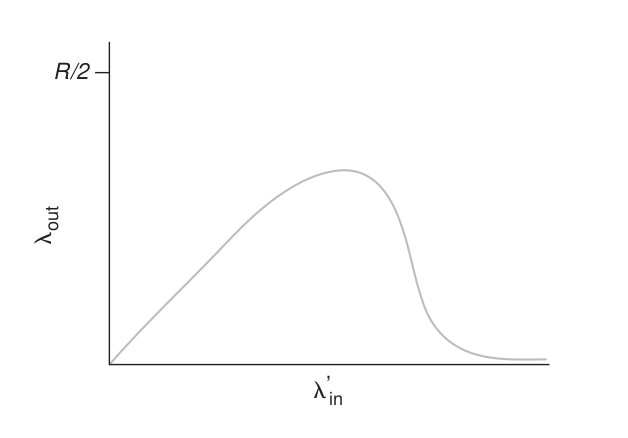
\includegraphics[scale=1,width=1\textwidth]{grafica_escenario_3.png}

\end{figure}

\subsection{Métodos para controlar la congestión de TCP}
Ya hemos visto que TCP proporciona un servicio de transporte fiable entre dos procesos que se ejecutan en hosts diferentes. Otro componente clave de TCP es su mecanismo de control de congestión. TCP tiene que utilizar un control de congestión terminal a terminal en lugar de un control de congestión asistido por la red, ya que la capa IP no proporciona una realimentación explícita a los sistemas terminales en lo tocante a la congestión de red. \\

El método empleado por TCP consiste en que cada emisor limite la velocidad a la que transmite el tráfico a través de su conexión en función de la congestión de red percibida. El mecanismo de control de congestión de TCP que opera en el emisor hace un seguimiento de una variable adicional, la ventana de congestión. Esta ventana, indicada como $VentCongestion$, impone una restricción sobre la velocidad a la que el emisor TCP puede enviar tráfico a la red. Específicamente, la cantidad de datos no reconocidos en un emisor no puede exceder el mínimo entre $VentCongestion$ y $VentRecepcion$, es decir:

\begin{equation*}
UltimoByteEnviado-UltimoByteReconocido \leq min\{VentCongestion, VentRecepcion\}
\end{equation*}

La restricción anterior limita la cantidad de datos no reconocidos por el emisor y, por tanto, limita de manera indirecto la velocidad de transmisión del emisor.  Definimos un 'suceso de pérdida' en un emisor TCP como el hecho de que se produzca un fin de temporización o se reciban tres paquete ACK duplicados procedentes del receptor. Cuando existe una congestión severa, entonces uno o más de los buffers de los routers existentes a lo largo de la ruta pueden desbordarse, dando lugar a que un datagrama sea descartado. A su vez, el datagrama descartado da lugar a un súceso de pérdida en el emisor, el cual lo interpreta como una indicación de que existe congestión en la ruta entre el emisor y el receptor. \\

Visto cómo se detecta la existencia de congestión en la red, vamos a considerar el mejor de los casos, cuando no existe congestión en la red, es decir, no se producen pérdidas de paquetes. En este caso, el emisor TCP recibirá todos los paquetes ACK correspondientes a los segmentos anteriormente no reconocidos. TCP interpretará esto como que todo va bien y empleará esos paquetes para incrementar el tamaño de la ventana de congestión. Obsérvese que si la velocidad de llegada de dichos paquetes es lenta, entonces el tamaño de la ventana de congestión aumenta a uno velocidad relativamente lenta. Puesto que TCP utiliza los paquetes ACK para provocar (o temporizar) sus incrementos del tamaño de la ventana de congesitón, se dice que TCP es \textbf{auto-temporizado}. \\

Para estudiar como un emisor TCP determina su velocidad de transmisión veremos los siguientes principios que TCP verifica:

\begin{itemize}
\item \textit{Un segmento perdido implica congestión y, por tanto, la velocidad del emisor TCP debe reducirse cuando se pierde un segmento.} 

\item \textit{Un segmento que ha sido reconocido indica que la red está estregando los segmentos del emisor al receptor y, por tanto, la velocidad de transmisión del emisor puede incrementarse cuando llega un paquete ACK correspondiente a un segmento que todavía no había sido reconocido.}

\item \textit{Tanteo del acho de banda.} Puesto que los paquetes ACK indican que la ruta está libre de congestión y la pérdida de paquetes indica que hay una ruta congestionada, la estrategia de TCP para ajustar su velocidad de transmisión consiste en incrementar su velocidad en respuesta a la llegada de paquetes ACK hasta que se produce una pérdida, momento en el que se reduce la velocidad de transmisión.
\end{itemize}

Conocidos los fundamentos del mecanismo de control de congestión TCP, estudiaremos el \textbf{algoritmo de control de congestión de TCP.} Este algoritmo consta de tres componententes principales: (1) arranque lento (\textit{slow start}),(2) evitación de la congestión (\textit{congestion avoidance}) y (3) recuperación rápida (\textit{fast recovery}). Los dos primero componentes son obligatorios en TCP, diferenciados en la forma en que aumentan el tamaño de la ventana de congestión en respuesta a los paquetes ACK recibidos. El componente recuperación rápida es recomendable, pero no obligatorio para emisores TCP.

\begin{figure}[h]
\centering
\caption{Descripción de la máquina de estados finitos del mecanismo de control de congestión de TCP}
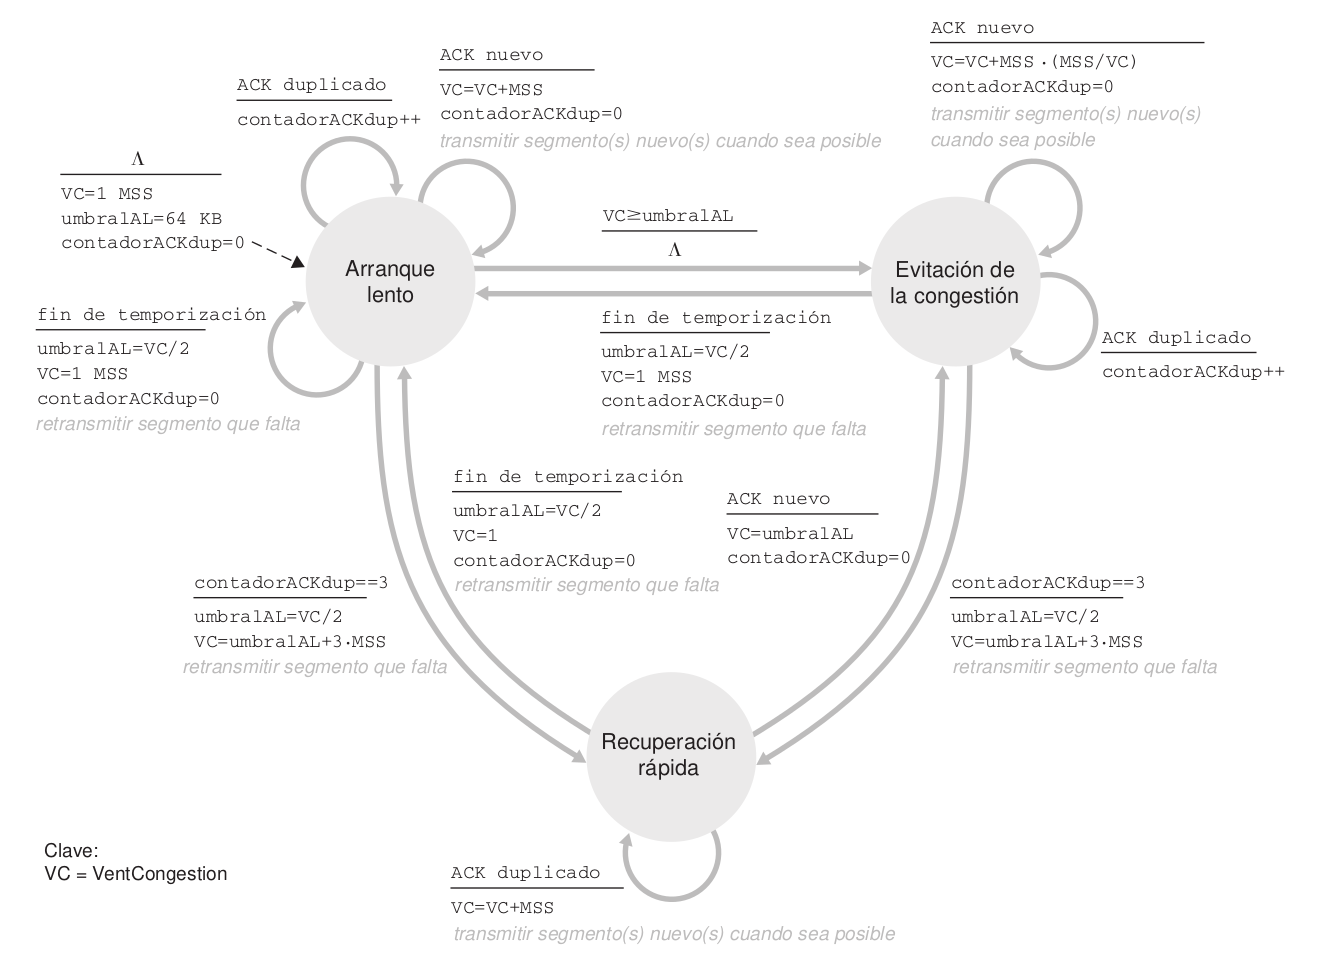
\includegraphics[scale=1,width=1.1\textwidth]{diagrama_estados_congestion.png}
\end{figure}

\subsection*{Arranque lento}
Cuando se inicia una conexión TCP, el valor de la ventana de congestión ($VentCongestion$) normalmente se incializa con un valor pequeño igual a 1 MSS, que da como resultado una velocidad de transmisión inicial aproximadamente igual a MSS/RTT. Puesto que el ancho de banda disponible para el emisor TCP puede ser mucho más grande que el valor MSS/RTT, al emisor TCP le gustaría poder determinar rápidamente la cantidad de ancho de banda disponible. Por lo tanto, en el estado de \textbf{arranque lento}, el valor de $VentCongestion$ se establece en 1 MSS y se incrementa un MSS cada vez que se produce el primer reconocimiento de un segmento transmitido.

\begin{figure}[h]
\centering
\caption{Fase de arrangue lento de TCP}
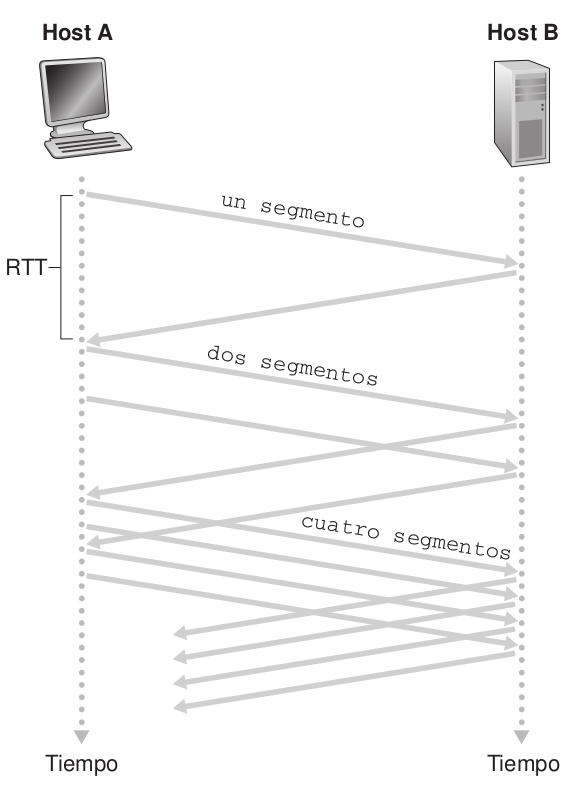
\includegraphics[scale=1,width=0.7\textwidth]{arranque_lento.png}
\end{figure}

El algoritmo de arranque lento proporciona varias respuesta para cuándo finalizar el crecimiento exponencial de la ventana de congestión. En primer lugar, si se produce un suceso de pérdida de paquete señalado por un fin de temporarización, el emisor TCP establece el valor de $VentCongestion$ en 1 e inicia de nuevo un proceso de arranque lento. También define el valor de una segunda variable de estado, $umblarAL$, que establece el umbral del arranque lento en $VentCongestion/2$, la mital del valor del tamaño de la ventana de congestión cuando se ha detectado que existe congestión. La segunda forma está directamente ligada al valor de $umbralAL$. Dado que $umbralAL$ es igual a la mitad del valor de $VentCongestion$ cuando se detectó congestión por última vez, puede resultar algo imprudente continuar duplicando el valor de $VentCongestion$ cuando se alcanza o sobrepasa el valor de umbral. Por tanto, cuando el valor de $VentCongestion$ es igual a $umbralAL$, la fase de arranque lento termina y las transacciones TCP pasan al modo de evitación de congestión. La última forma en la que puede terminar la fase de arranque lento es si se detectan tres paquetes ACK duplicados, en cuyo caso TCP realiza un retransmisión rápida y entra en el estado de recuperación rápida.

\subsection*{Evitación de la congestión}
Al entrar en el estado de evitación de congestión, el valor de $VentCongestion$ es aproximadamente igual a la mitad de su valor en el momento en que se detectó congestión por última vez. En consecuencia, en lugar de duplicar el valor de $VentCongestion$ para cada RTT, TCP adopta un método más conservador e incrementa el valor de $VentCongestion$ solamente en un MSS cada RTT. Esto se puede llevar a cabo de varias maneras. Un método habitual consiste en que un emisor TCP aumenta el valor de $VentCongestion$ en MSS bytes cuando llega un nuevo paquete de reconocimiento (se considera paquete de reconocimiento tanto ACK como segmento se envian en un RTT). El algoritmo de evitación de la congestión de TCP se comporta del mismo modo que cuando tiene lugar un fin de temporización. Como en el caso del modo de arranque lento, el valor de $VentCongestion$ se fija en 1 MSS y el valor de umbralAL se actualiza haciéndose igual a la mitad del valor de $VentCongestion$ cuando se produce un suceso de pérdida de paquete. Sin embarigo, recuerde que también puede detectarse una pérdida de paquete a causa de la llegada de tres ACK duplicados. En este caso, la red continúa entregando segmento del emisor al receptor. Por tanto, el comportamiento de TCP ante este tipo de pérdida debería ser menos drástico que ante una pérdida de paquete indicada por un fin de temporización: TCP divide entre dos el valor de $VentCongestion$ (añadiendo 3MSS como forma de tener en cuenta los tres ACK duplicados que se han recibido) y configura el valor de $umbralAL$ para que sea igual a la mita del valor que $VentCongetion$ tenía cuando se recibieron los tres ACK duplicados. A continuación, se entra en el estado de recuperación rápidad.

\subsection*{Recuperación rápida}
Enla fase de recuperación rápida, el valor de $VentCongestion$ se incrementa en 1 MSS por cada ACK duplicado recibido correspondiente al segmento que falta y que ha causado que TCP entre en el estado de recuperación rápida. Cuando llega un ACK para el segmento que falta, TCP entra de nuevo en el estado de evitación de la congestión después de disminuir el valor de $VentCongestion$. Si se produce un fin de temporización, el mecanismo de recuperación rápida efectúa una transición al estado de arranque lento después de realizar las mismas acciones que en los modos de arranque lento y de evitación de la congestión: el valor de $VentCongestion$ se establece en 1 MSS y el valor de $umbralAL$ se hace igual a la mitad del valor que tenía $VentCongestion$ cuando tuvo lugar el suceso de pérdida. \\

Ya se ha dicho que el mecanismo de recuperación rápida no es un componente obligatorio. Es interesante resaltar que una versión anterior de TCP, conocida como TCP Tahoe, establece incondicionalmente el tamaño de la ventana de congestión en 1 MSS y entra en el estado de arranque lento depués de un suceso de pérdida indicado por un fin de temporización o por la recepción de tres ACK duplicados. La versión más reciente de TCP, TCP Reno, incorpora la recuperación rápida.

\begin{figure}[h]
\centering
\caption{Evolución de la ventana de congestión de TCP (Tahoe y Reno)}
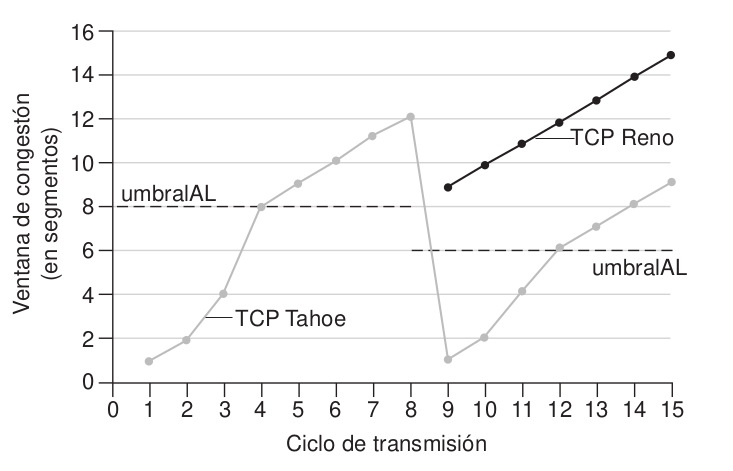
\includegraphics[scale=1,width=0.8\textwidth]{tcp_tahoe_reno.png}
\end{figure}

\section{Extensiones TCP}
Existen muchos tipos de TCP, lo que se concoe como sabores de TCP, que viene de flavour en inglés, es decir, versiones. Todos ofrecen una interoperabilidad, ya que tiene que convivir con el resto de TCP que existen. \\

Para cualquier versión de Linux con kernel mayor que la 2.6.19, se usa la versión de TCP 'TCP CuBIC', que a su vez, tiene también varias versiones. Esta versión de TCP tiene una especie de temporizador para pegarse lo más posible al límite de la red.

\begin{figure}[h]
\centering
\caption{Ventana de congestión dinámica de TCP CuBIC}
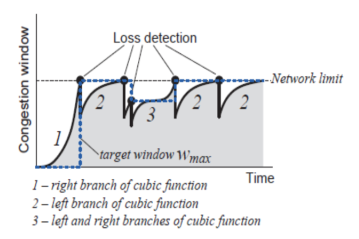
\includegraphics[scale=1,width=0.8\textwidth]{ventana_congestion.png}
\end{figure}

Por otro lado en la figura 23 podemos ver las distintas familias de TCP que existen. En cada isla podemos ver un tipo distinto de TCP, y varían unas de otras en función del SO, del tipo de red (ya que un TCP de una red inalámbrica tiene unas característica distintas de otro TCP que funciona sobre una red cableada). \\

\begin{figure}[h]
\centering
\caption{Arbol con familias de TCP según su Control de Congestión}
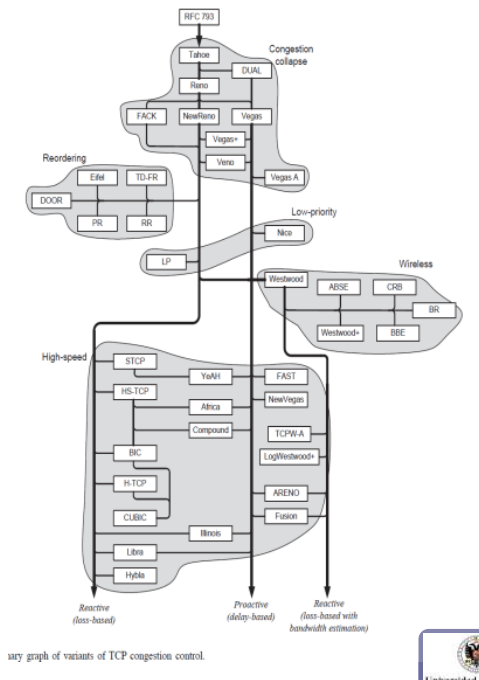
\includegraphics[scale=1,width=0.8\textwidth]{familias_tcp.png}
\end{figure}

De todas las familias existentes, hay una serie de extensiones que tienen muchos tipos de TCP actuales, estas son las más importantes:

\begin{itemize}
\item \textbf{Ventana escalada:} el campo \textit{window} es de 2 bytes, esto significa que como máximo se tiene una ventana de $2^{16}-1$. Esta ventana, en una situación en la que se use una red moderna, una en la que pueda haber una velocidad de 1Gb/s, el tiempo de transmisión es muy pequeño. Eso con un tamaño de ventana limitado como máximo a $2^{16}-1$ puede hacer que se produzcan tiempos muertos muy grandes, ya que un paquete se envía muy rápido, pero el tiempo de propagación es muy lento. Incluso aumentando el número de paquetes que se envían, se seguirán teniendo tiempos muertos muy grandes. \\

Por lo que para redes modernas se necesita ampliar el tamaño de ventan para poder conseguir el rendimiento de la eficiencia unidad. Esto sucede cuando el tiempo de transmisión se reduce muchísimos, y lo que manda es el tiempo de propagación. De hecho, llegar a conseguir la eficiencia unidad cuesta mucho más cuando crezca el tiempo de propagación respecto al de transmisión. \\

Con las redes muy amplias, se necesitan ventanas muy amplias. Por eso, una de las opciones que se añaden durante el hanshake es habilitar la ventana escalada en la cabecera, lo que contiene un factor de escala por el que se multiplica la ventana máxima. Este factor de escala utiliza una ley exponencial. Este valor de escala puede llegar a $2^{14}$. Esto junto a los $2^16$ bytes que había inicialmente, hacen un total de $2^{30}$ bytes, es decir, se puede llegar a conseguir una ventana de 1GB. Con este tamaño de ventana, es más fácil llegar al rendimiento de la eficiencia unidad. 

\item \textbf{Estimación RTT:} esta estimación RTT consiste en que al enviar un segmento, se mete dentro del paquete un sello de tiempo (\textit{time stamp}), es decir, el momento de tiempo justo en el que lo está enviando. Cuando responda con un ACK, este ACK también tendrá un sello de tiempo, aunque también puede tener registrado este tiempo, en vez de tener que llevarlo el ACK. Si se manda un paquete con un sello de tiempo X, el ACK que se espera tendrá también el sello de tiempo $X_1$. Cuando llegue el ACK, lo único que hay que hacer es restar ambos sellos, con lo que se consigue estimar el RTT, sin necesidad de comprobar que llega al ACK del siguiente, etc. \\

Esto también sirve para que cuando llegue un segmento con un time stamp que ya ha pasado, se desprecie directamente, ya que no es información útil. Esto se conoce como los PAWS (\textit{Protect Against Wrapped Sequence numbers}). 

\item \textbf{SACKS o confirmaciones selectivas:} antes se tenían ACK's acumulativos, es decir, si llegaba un ACK con número de secuencia X, se confirmaba todo lo que había antes de ese ACK. El problema de esto es que si este ACK no llega, tiene que reenviarse todo desde lo que no ha llegado. Existe una forma (\textit{Selective Acknowledgment}) que permite que el receptor confirme uno de los segmentos que haya en juego. Un ejemplo, es que si se tienen tres segmentos en juegos, a la espera de ser confirmados, el receptor puede confirmar uno de los paquetes, independientemente de los dos anteriores no le hayan llegado, como se confirma de forma selectiva, es decir, lo que ha llegado, el emisor también lo entiende de forma selectiva, por lo que hay que reenviar alguno de los otros dos paquetes, se envía el que falte. Es una forma de evitar los reenvios innecesarios.
\end{itemize}



\section{Glosario:}
\begin{itemize}
\item \textbf{Primitivas de transporte:} operación que la capa de transporte ofrece a los programas de aplicación.
\end{itemize}



\end{document}